\section{Adaptive Music System}

In the year 2019, the authors Patrick Hutchings and Jon McCormack
introduced the Adaptive Music System (AMS) \cite{hutMcCormAms} 
and tested it with several evaluators. It was developed as a
stand-alone package that receives game information from the
video game itself in real-time to generate a model of the game-
state and output music from this state \cite{hutMcCormAms}.
Their system is divided into two main components: 
\begin{enumerate}[label=\arabic*)]
    \item A spreading activation model to read the game's information \cite{hutMcCormAms}.
    \item The music generation system that uses the spreading activation model output to generate its music \cite{hutMcCormAms}. 
\end{enumerate}

\begin{figure}[h]
    \centering
    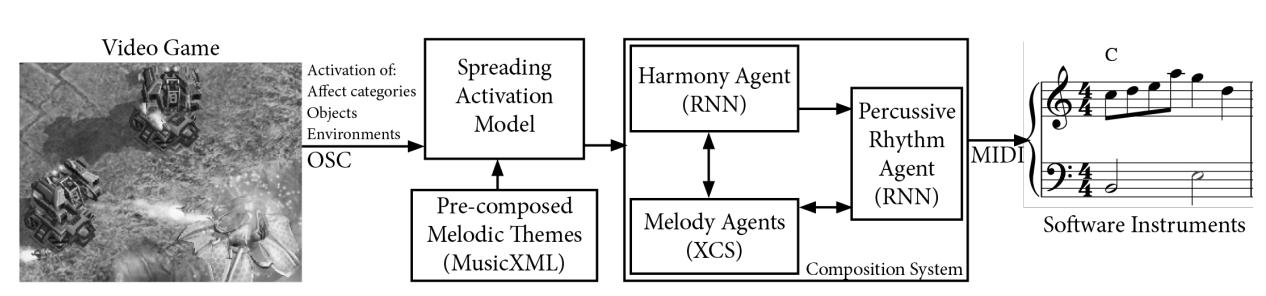
\includegraphics[width=\linewidth]{images/ams_architecture.png}
    \caption{Architecure of AMS \cite{hutMcCormAms}}
    \label{fig:ams_architecture}
\end{figure}

A first introduction of the system can be seen in \Cref{fig:ams_architecture}.
It represents the whole workflow of music generation \cite{hutMcCormAms}. The game 
acts here as an input for the Spreading Activation Model, which passes its output
to the music Composition System \cite{hutMcCormAms}. The system outputs music in
MIDI format \cite{hutMcCormAms}. MIDI (Musical Instrument Digital Interface) is a
common music format \cite{midi_explanation} that can also be used as a protocol
between computers and synthesizers \cite{midi_explanation}. It can be also used to 
generate synthesized music \cite{midi_explanation} with many types of instruments \cite{midi_general}.

The MIDI files are then used to generate Music with specific software systems \cite{hutMcCormAms}.



\subsection{Spreading Activation Model}

The spreading activation model \cite{collins1975spreading} itself is a knowledge 
organisation model, which can be used to understand and capture emotion \cite{hutMcCormAms}\cite{carr1982words} in a graph, making it 
worth being used in a video game \cite{hutMcCormAms}.

For the AMS, the authors described the implementation
of the spreading activation model as a weighted and 
undirected graph \( G = (V, E) \)\cite{hutMcCormAms}, where 
\( V \) represents the vertices, and \( E \) the edges of the
graph. Each node \( V \) of the graph 
stands for a certain context \cite{hutMcCormAms}, which can
be either an affect \( (A) \), an  \( (O) \) object or an environment \( (N) \) \cite{hutMcCormAms}. A node
contains an activation value from 0 to 100 \cite{hutMcCormAms}. The 
edges of the graph stand for the level of  association 
of those context objects \cite{hutMcCormAms} 
and have normalised weights \( w_E\). Nevertheless, the authors
say that the nodes do not have to be connected, and edges do not 
form between affects \cite{hutMcCormAms}. 

Initially at the game
start, the graph contains the affect nodes sadness, happiness, 
threat, anger, tenderness and excitement \cite{hutMcCormAms}
and receives updates from the game every 30ms \cite{hutMcCormAms}.
The model uses an Open Sound Control (OSC) client to refresh
the graph with the game information, and nodes are newly generated
when a concept is not contained within the graph.

Nodes which contain a positive activation level are able to activate
adjacent nodes \cite{hutMcCormAms}. The activation done proportionally to the weights
of the edges \cite{hutMcCormAms}. For instance, if a Node A has an activation level
of 50 and has an adjacent node B, connected with an edge weight
of 0.25, Node A will activate Node B with at least 12.5 \cite{hutMcCormAms}. If
the Node has already been activated with the same or a higher
value, the vertex weight stays the same. To conclude, the activation
can be described as \[
w_B := 
\begin{cases} 
w_A * w_E & \text{if } w_A * w_E > w_B \\
w_B & \text{if not} 
\end{cases}
\] 
where \( (w_A) \) is the activation value of vertex A, \(( w_B )\)
is the activation of vertex B and \( (w_E) \) is the normalised value
of the edge connecting both vertices together.


\subsection{Music Composition System}

